\documentclass{beamer}
\usepackage[utf8]{inputenc}
\usepackage[frenchb]{babel}
\usepackage{tikz}
\usepackage{subfigure}
\usepackage[scriptsize]{caption}
\usepackage{multicol}
\usepackage{lipsum}
\renewcommand*{\figurename}{}
\usetikzlibrary{shapes,positioning,snakes,calc}
\usetheme{Warsaw}

% \setbeamercolor{alerted text}{fg=blue}

\def\android{Android\texttrademark}

\title{FMIN200 \\ TER~: Reconception du jeu PtiClic sous \android{}}
\author{DUPÉRON Georges \and\\ CHARRON John \and\\ BRUN Bertrand \and\\ BONAVERO Yoann}
\institute{Université Montpellier II, Département informatique}
\date{Jeudi, 26 mai 2011}

\defbeamertemplate*{footline}{shadow theme}
{%
  \leavevmode%
  \hbox{\begin{beamercolorbox}[wd=.5\paperwidth,ht=2.5ex,dp=1.125ex,leftskip=.3cm plus1fil,rightskip=.3cm]{author in head/foot}%
    \usebeamerfont{author in head/foot}\insertframenumber\,/\,\inserttotalframenumber\hfill\url{http://pticlic.fr/}
  \end{beamercolorbox}%
  \begin{beamercolorbox}[wd=.5\paperwidth,ht=2.5ex,dp=1.125ex,leftskip=.3cm,rightskip=.3cm plus1fil]{title in head/foot}%
    \usebeamerfont{title in head/foot}\insertshorttitle%
  \end{beamercolorbox}}%
  \vskip0pt%
}

\begin{document}

\begin{frame}
  \titlepage
\end{frame}

% John
\section{Introduction}

\begin{frame}  
\begin{figure}[h!]
  \centering
      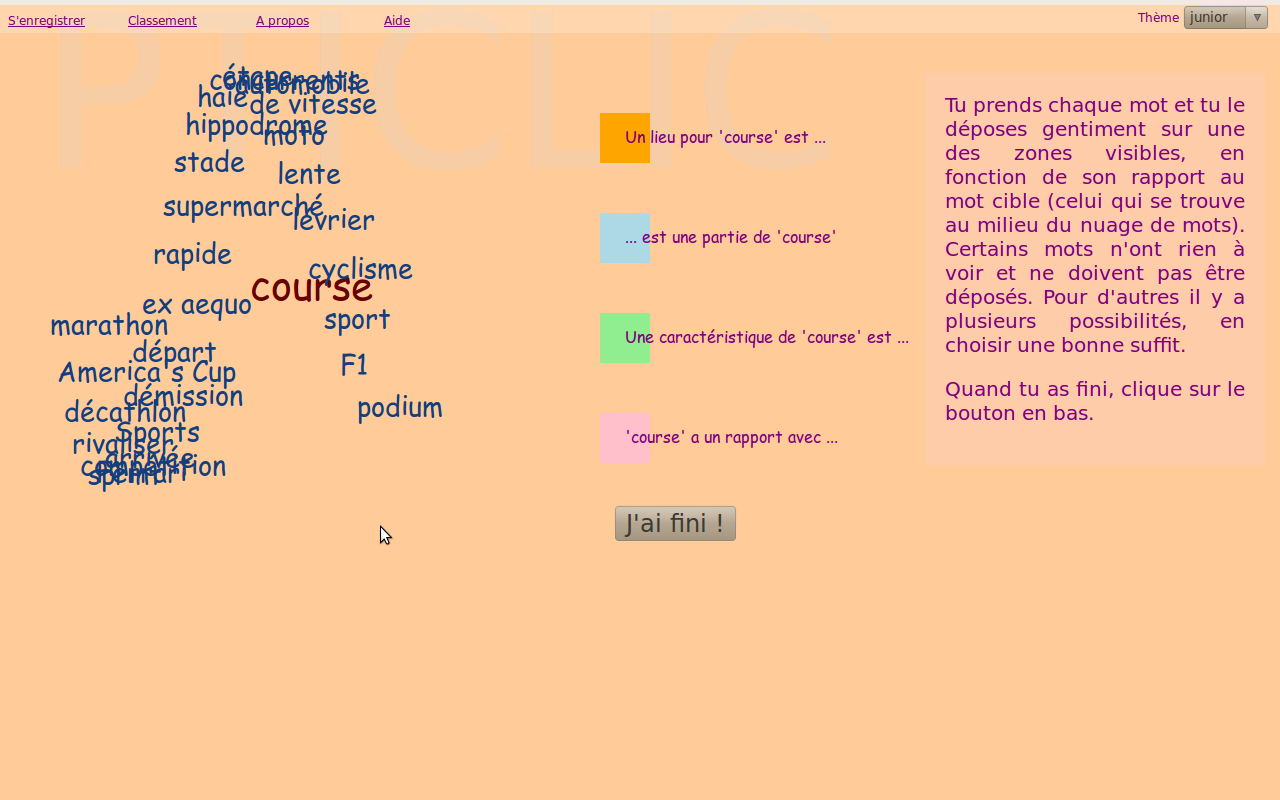
\includegraphics[width=0.8\textwidth]{img/PtiClicJeu.png}
\caption{PtiClic de Mathieu LAFOURCADE et Virginie ZAMPA}
\end{figure}
\end{frame}

\begin{frame}  
\begin{figure}[h!]
  \centering
      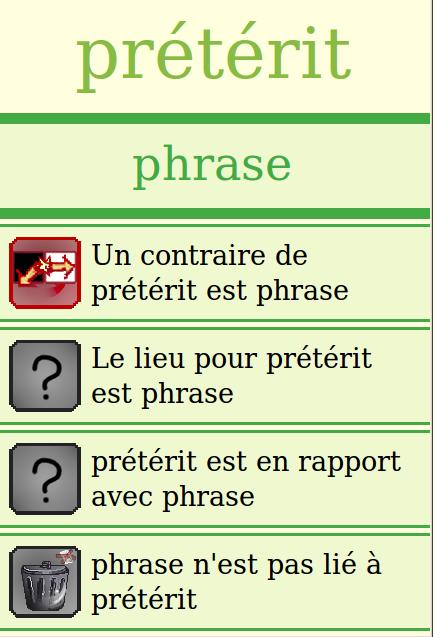
\includegraphics[width=0.4\textwidth]{img/preterit01.jpg}
\caption{Reconception PtiClic Version HTML5}
\end{figure}
\end{frame}

\begin{frame}  
\begin{figure}[h!]
  \centering
      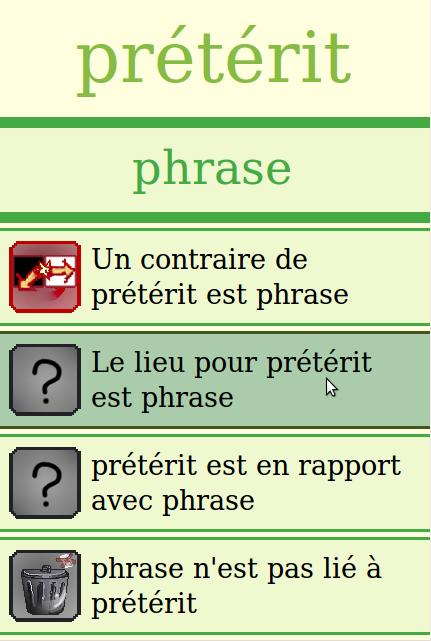
\includegraphics[width=0.4\textwidth]{img/preterit02.jpg}
\caption{Reconception PtiClic Version HTML5}
\end{figure}
\end{frame}

\begin{frame}  
\begin{figure}[h!]
  \centering
      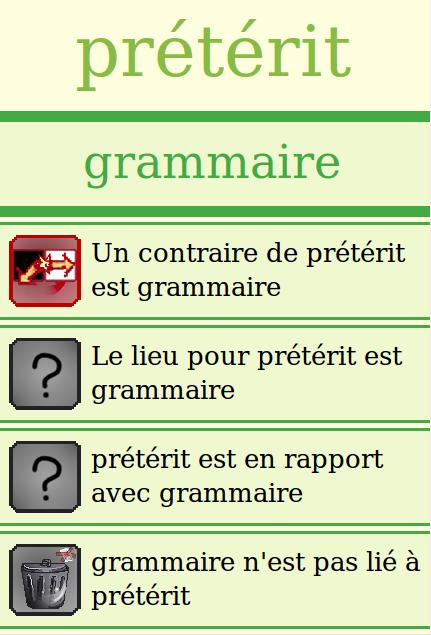
\includegraphics[width=0.4\textwidth]{img/preterit03.jpg}
\caption{Reconception PtiClic Version HTML5}
\end{figure}
\end{frame}

\begin{frame}  
\begin{figure}[h!]
  \centering
      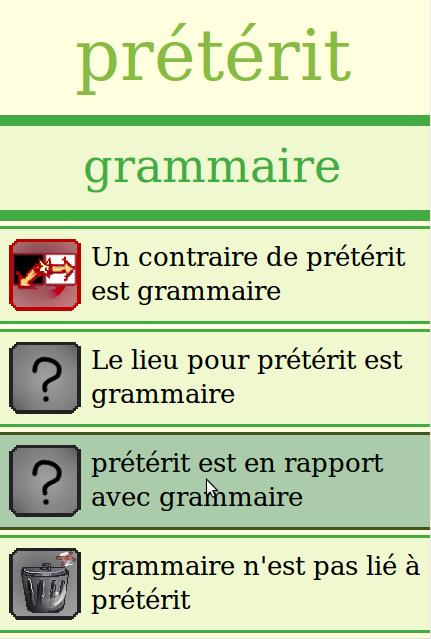
\includegraphics[width=0.4\textwidth]{img/preterit04.jpg}
\caption{Reconception PtiClic Version HTML5}
\end{figure}
\end{frame}

\begin{frame}  
\begin{figure}[h!]
  \centering
      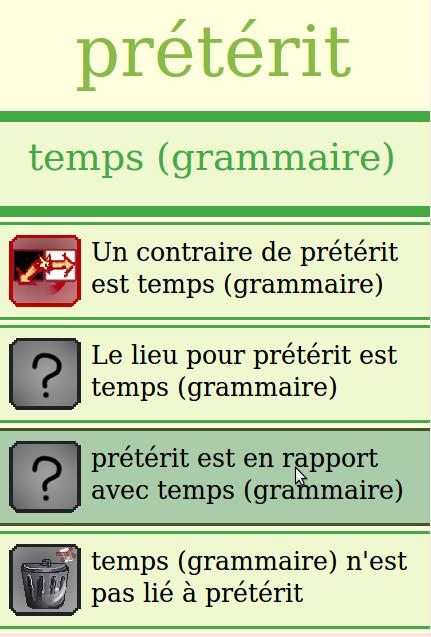
\includegraphics[width=0.4\textwidth]{img/preterit05.jpg}
\caption{Reconception PtiClic Version HTML5}
\end{figure}
\end{frame}

\begin{frame}  
\begin{figure}[h!]
  \centering
      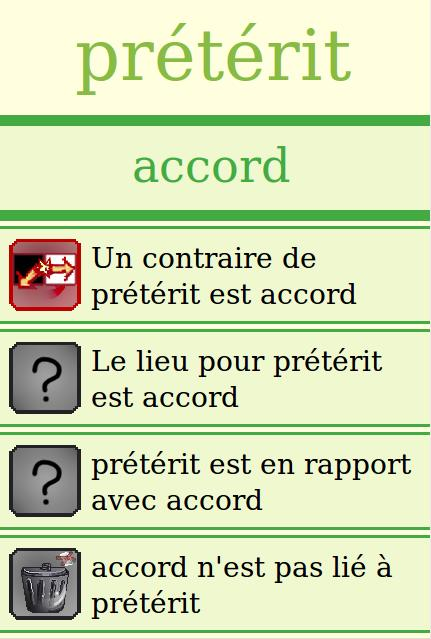
\includegraphics[width=0.4\textwidth]{img/preterit06.jpg}
\caption{Reconception PtiClic Version HTML5}
\end{figure}
\end{frame}

\begin{frame}  
\begin{figure}[h!]
  \centering
      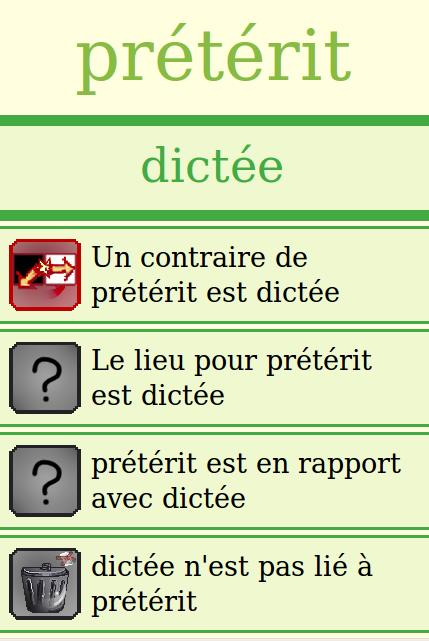
\includegraphics[width=0.4\textwidth]{img/preterit07.jpg}
\caption{Reconception PtiClic Version HTML5}
\end{figure}
\end{frame}

\begin{frame}  
\begin{figure}[h!]
  \centering
      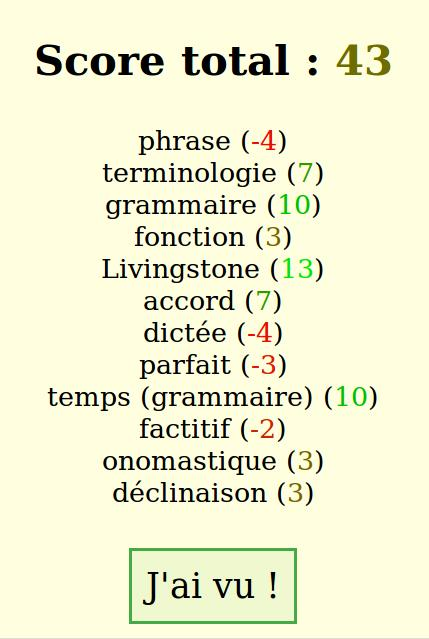
\includegraphics[width=0.4\textwidth]{img/preterit08.jpg}
\caption{Reconception PtiClic Version HTML5}
\end{figure}
\end{frame}



\section{Paquetage TALN}

\begin{frame}
  Ferdinand de Saussure (1857-1913), Cours de linguistique générale
  \begin{itemize}
  \item Signe linguistique

  \begin{figure}
\centering
\mbox{
\subfigure{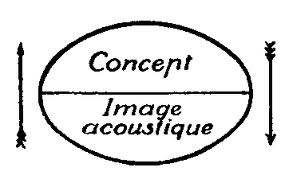
\includegraphics[scale=0.3]{img/signe-conceptimageacoustique.jpeg}}\quad
\subfigure{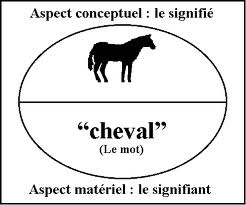
\includegraphics[scale=0.3]{img/signe-cheval.jpeg}}\quad
\subfigure{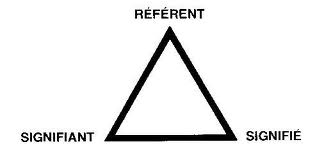
\includegraphics[scale=0.3]{img/trianglesemiotique.jpeg}}
}
\end{figure}
  
\item Arbitraire du signe
  \item Synchronie et Diachronie
  \item Langue et Parole
  \end{itemize}
  
\end{frame}

\begin{frame}
\begin{center}
  Réseau lexical JeuxDeMots  \\\
  \end{center}

Types de noeuds
  \begin{itemize}
  \item termes
  \item catégories grammaticales
  \item informations métalinguistiques supplémentaires 
  \end{itemize}

  \textcolor{white}{text}\\
  Types de relations 
  \begin{itemize}
  \item morphologique
  \item sémantique
  \item métalinguistique
  \end{itemize}
  
\end{frame}

\begin{frame}
  Réseau lexical JeuxDeMots~: quelques statistiques
  \begin{itemize}
  \item environ 45\% des noeuds n'ont pas de relations sémantiques sortantes
  \item environ 70\% des noeuds n'ont pas de relations sémantiques entrantes
  \end{itemize}
\end{frame}

\begin{frame}
  Réseau lexical JeuxDeMots~: bruits et silences
  \begin{itemize}
  \item bruits = relations plus fortes que la réalité 
  \item silence = relations non existantes ou trop faible par rapport à la réalité 
  \item bruits + silences = couverture de relations sémantiques hétérogènes
  \end{itemize}
\end{frame}

\begin{frame}
\begin{figure}
  \begin{center}
    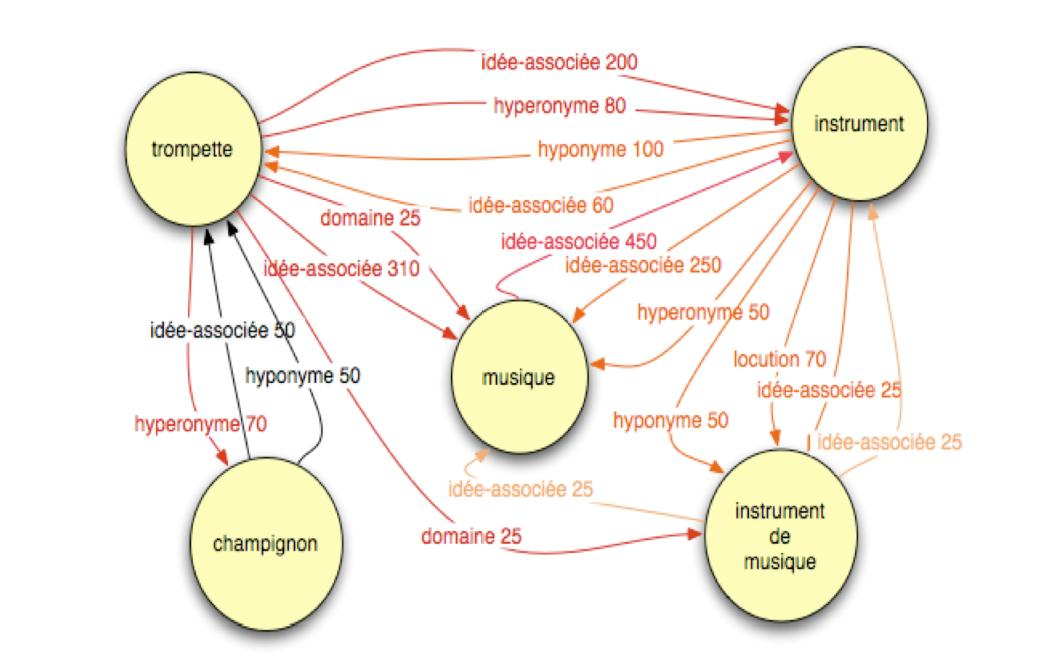
\includegraphics[width=0.75\textwidth]{img/jdm.jpeg}
  \end{center}
\end{figure}
\end{frame}

\begin{frame}
\begin{center}
	\begin{tabular}{ | l | l | l | l | p{5cm} |}
        \hline
\footnotesize{Relation} & \footnotesize{Mot central} & \footnotesize{Mots nuage} & \footnotesize{Remarques} \\ \hline
\footnotesize{-1 'mn' n'est pas lié à 'mc'} & \footnotesize{\shortstack{adj adv n v}} & \footnotesize{\shortstack{adj adv n v}} & \footnotesize{} \\ \hline
\footnotesize{0 'mc' est en rapport avec 'mn'} & \footnotesize{\shortstack{adj adv n v}} & \footnotesize{\shortstack{adj adv n v}} & \footnotesize{} \\ \hline
\footnotesize{5 'mc' est un synonyme de 'mn'} & \footnotesize{\shortstack{adj adv n v}} & \footnotesize{\shortstack{adj adv n v}} & \footnotesize{\shortstack{même POS}} \\ \hline
\footnotesize{6 'mc' est une sorte de 'mn'} & \footnotesize{n} & \footnotesize{n} & \footnotesize{} \\ \hline
\footnotesize{7 Un contraire de 'mc' est 'mn'} & \footnotesize{\shortstack{adj adv n v}} & \footnotesize{\shortstack{adj adv n v}} & \footnotesize{\shortstack{même POS}} \\ \hline
\footnotesize{8 Un spécifique de 'mc' est 'mn'} & \footnotesize{n} & \footnotesize{n} & \footnotesize{} \\ \hline
\footnotesize{9 'mn' est une partie de 'mc'} & \footnotesize{n} & \footnotesize{n} & \footnotesize{} \\ \hline
\footnotesize{10 'mc' fait partie de 'mn'} & \footnotesize{n} & \footnotesize{n} & \footnotesize{} \\ \hline
\footnotesize{13 'mn' pourrait 'mc'} & \footnotesize{v} & \footnotesize{n} & \footnotesize{} \\ \hline
\footnotesize{15 Le lieu pour 'mc' est 'mn'} & \footnotesize{n v} & \footnotesize{\shortstack{n}} & \footnotesize{} \\ \hline
\footnotesize{16 Instrument pour 'mc' est 'mn'} & \footnotesize{v} & \footnotesize{n} & \footnotesize{} \\ \hline
\footnotesize{17 'mn' Caractéristique de 'mc'} & \footnotesize{n} & \footnotesize{adj} & \footnotesize{} \\ \hline
        \end{tabular}
\end{center}
\end{frame}

\begin{frame}
  \begin{figure}
    \pgfdeclarelayer{background}
    \pgfdeclarelayer{foreground}
    \pgfsetlayers{background,main,foreground}
    \begin{tikzpicture}[
      txt/.style = {fill=white,font=\footnotesize,scale=0.75, inner sep=1pt},
      earlymidway/.style = {pos=0.4},
      latemidway/.style = {pos=0.6}
      ]
      \node (n0) {musique};
      \node[above left  = 2cm of n0] (n1) {trompette};
      \node[above right = 2cm of n0] (n2) {instrument};
      \node[below left  = 2cm of n0] (n3) {champignon};
      \node[below right = 2cm of n0] (n4) {instrument de musique};
      
      \foreach \direction/\nfrom/\nto/\angle/\pos/\anchor/\text in {
        ->/n0/n2/15/near end/east/idée associée 450,
        <-/n0/n2/0/midway/center/idée associée 250,
        <-/n0/n2/-15/near start/west/hyperonyme 50,
        % 
        ->/n0/n4/-20/midway/center/idée associée 25,
        % 
        ->/n2/n4/-15/near end/east/hyponyme 50,
        ->/n2/n4/0/latemidway/east/locution 70,
        ->/n2/n4/15/latemidway/west/idée associée 25,
        <-/n2/n4/30/near end/west/idée associée 25,
        % 
        ->/n1/n3/-15/very near end/east/hyperonyme 70,
        <-/n1/n3/0/latemidway/center/idée associée 50,
        <-/n1/n3/15/very near end/west/hyperonyme 50
      }{
        \draw[\direction] (\nfrom) to[bend left=\angle] (\nto);
        \begin{pgfonlayer}{foreground}
          \path[\direction] (\nfrom) to[bend left=\angle] node[\pos, anchor=\anchor, txt] {\text} (\nto);
        \end{pgfonlayer}
      }
    \end{tikzpicture}
  \end{figure}
\end{frame}

\begin{frame}
  Pas de conflit de relations et la bonne catégorie grammaticale~: conditions nécessaires mais pas suffisantes 
  \begin{itemize}
  \item 'mn' est une partie de 'mc'~: les mots doivent être des noms, mais doivent aussi être des choses physiques. Le mot "honnêteté' ne marchera pas
  \item 'mn' pourrait 'mc' (Qui/Quoi pourrait 'mc')~: les mots doivent être des noms et un verbe respectivement, mais un verbe d'état ne conviendrait pas
  \item le lieu de 'mc' est 'mn'~: les mots doivent être un nom ou verbe puis un nom, mais le nom doit pouvoir signifier un lieu, un endroit
Il existe un dispositif dans la base de données prévu pour nous donner des informations métalinguistiques afin de faire ses distinctions, mais souvent la base n'est pas suffisemment alimentées pour pouvoir exploiter ces attributs sémantiques.
  \end{itemize} 
\end{frame}


\begin{frame}
  Algorithme de base pour introduire des mots sans aucune relation sémantique 
  \begin{enumerate}
  \item On génère le nuage à l'aide d'une méthode ou algorithme auxiliaire (LSA ou autre) à partir d'un mot central choisi au hasard
  \item On choisit la seule relation sémantique "idée associée" afin de valider les mots générés par l'étape précédente (ainsi on établit des relations sortantes "idée associée" à partir d'un mot)
  \item Algorithme suivant sera utilisé pour affiner les informations concernant le mot central en question
  \end{enumerate} 
\end{frame}


\begin{frame}
LSA ou autres méthodes d'établir des liens sémantiques
\begin{figure}
 \begin{minipage}{\textwidth}
\centering 
       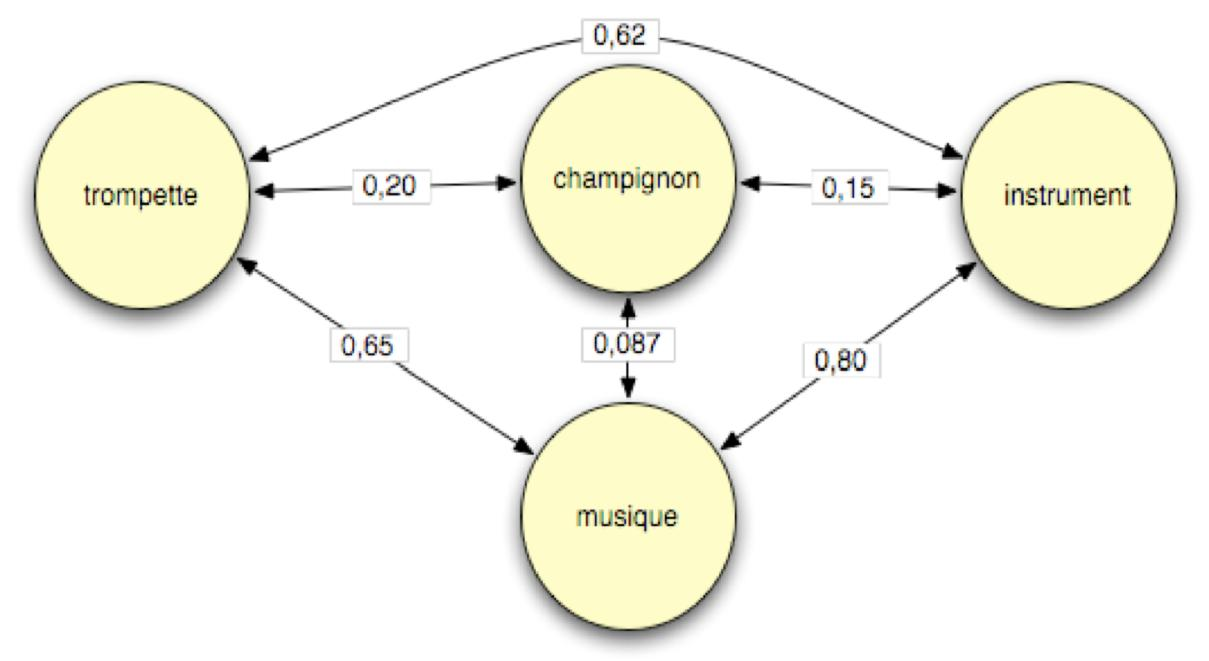
\includegraphics[width=0.75\textwidth]{img/lsa.jpeg}
  \end{minipage}
\end{figure}
\end{frame}

\begin{frame}
  Algorithme pour affiner des relations de types "idée associée"
  \begin{enumerate}
  \item On génère le nuage à partir de la relation sémantique le plus général, quasiment toutes les autres relations sémantiques étant un sous-ensemble de cette relation
  \item On choisit des relations sémantiques plus spécifiques sans conflits (tableau "relations" précédent)
  \end{enumerate}  
\end{frame}

\begin{frame}
  Algorithme pour renforcer ajouter et renforcer des relations sémantiques spécifiques, quelques exemples
\begin{itemize}
\item Pour la relation de synonymie, on génère des mots nuage "synonyme de synonyme" ou bien "antonyme d'antonyme" du mot central
\item Pour la relation d'antonymie, on génère des mots nuage "antonyme de synonyme" ou bien "synonyme d'antonyme" du mot central
\item Pour la relation "spécifique de" on bascule une fois entre "est une sorte de" et "est un spécifique du" mot central une fois (et inversement dans le cas inverse, on peut aussi appliquer le même principe aux relations contenu/contenant, etc.
\end{itemize}
Inconvénient~: on n'introduit pas de nouvelles relations sémantiques spécifiques et le renforcement est possible à l'aide de l'algorithme du transparent précédent
\end{frame}

\section{Generation de partie}

\begin{frame}
  % Georges
  \begin{tikzpicture}[
    mynode/.style = {circle, minimum size=1.5cm},
    mc/.style = {mynode,draw=red,text=red},
    mn/.style = {mynode,draw},
    mi/.style = {mynode,draw=gray,text=gray},
    rel/.style = {font=\footnotesize},
    guess/.style = {->,dashed},
    exist/.style = {->},
    auto,swap
    ]
    \node[mc] (mc) {Chat};
    \node[mn] (mn0) at (0,3) {Souris};
    \node[mi] (mi1) at (3,-2) {matou};
    \node[mn] (mn2) at (6,0) {animal};
    \path[exist] (mc) edge[bend right] node[rel]{idée associée} (mn0);
    \path[exist] (mc) edge node[rel]{synonyme} (mi1);
    \path[exist] (mi1) edge node[rel]{sorte de} (mn2);
    \path[guess,swap] (mc) edge node[rel]{sorte de ?} (mn2);
    \path[guess,swap] (mc) edge[bend left] node[rel]{\shortstack{sorte de ?\\synonyme ?\\\dots}} (mn0);
  \end{tikzpicture}
\end{frame}

% bertrand
\section{Le Jeu}

\begin{frame}
\frametitle{Le framework \android{}}
\begin{block}{Les outils mis à disposition}
  \begin{itemize}
    \item<+-> Langage de programmation Java ;
    \item<+-> Patron de conception MVC (Modèle-Vue-Contrôlleur);
    \item<+-> Les vues sont réalisé en XML
  \end{itemize}
\end{block}
\begin{alertblock}{Inconvenient}<+->
  L'édition des vues en XML nous à énorment ralenti lors du développement de l'alpha 1
\end{alertblock}
\end{frame}

\begin{frame}
\frametitle{Le modèle MVC proposé par Google}
\begin{block}{Modèle-Vue-Contrôlleur}
  \centering
  \begin{tikzpicture}[bend angle=10, shorten >=0.1cm, shorten <=0.1cm]
    \node[draw] (activite) {Activité};
    \node[draw,below right=of activite] (modele) {Modèle};
    \node[draw,below left=of activite] (xml) {Vue (XML)};
    \draw[->] (activite.east) ++(0,+.1cm) to[out=0,   in=90] ($(modele.north)+(+.1cm,0)$);
    \draw[<-] (activite.east) ++(0,-.1cm) to[out=0,   in=90] ($(modele.north)+(-.1cm,0)$);
    \draw[->] (activite.west) ++(0,+.1cm) to[out=180, in=90] ($(xml.north)+(-.1cm,0)$);
    \draw[<-] (activite.west) ++(0,-.1cm) to[out=180, in=90] ($(xml.north)+(+.1cm,0)$);
  \end{tikzpicture}
\end{block}
\begin{block}{Détail}
\begin{description}
  \item[Modèle] Classe metier permettant de stocker des informations
  \item[Contrôlleur] Classe héritant d'\verb!Activity! (Activité)
  \item[Vue] XML affichant les informations
\end{description}
\end{block}
\end{frame}

\begin{frame} % Un peu vide peut etre ajouter les autre activite tel que prefs, info...
\frametitle{Prototype 1}
 \begin{block}{Schéma générale de l'enchainement des Activités~:}
   \centering 
  \begin{tikzpicture}[
    state/.style={draw},
    transition/.style={->}
    ]
    \node[state] (frontpage) {Page de garde};
    \node[state, right=of frontpage] (game) {Jeu};
    \node[state, right=of game] (score) {Score};
    
    \draw[transition] (frontpage) -- (game);
    \draw[transition] (game) -- (score);
    \draw[transition] (score.south) -- ++(0,-0.3cm) -| (frontpage);
    \draw[transition,<-] (game.north) -- ++(0,0.3cm) -| ($.5*(game) + .5*(score)$);
    
    \node[state,text width=1.2cm, below=of frontpage] (activite) {Activité};
    \draw[transition] (activite.north east) ++(0.5cm,0) -- node[auto,swap,font=\footnotesize,scale=0.8] {\shortstack{\shortstack{Évènement\\(Intent)}}} ++(1.5cm,0);
  \end{tikzpicture}
 \end{block}
\end{frame}

\begin{frame}
\frametitle{Passage au HTML}
\begin{block}{Défauts constatés}
  \begin{itemize}
    \item<+-> Perte de temps avec les ajustements des vues ;
    \item<+-> Public visé trop faible ;
  \end{itemize}
\end{block}
\begin{block}{Solutions proposées}<+->
  \begin{itemize}
    \item<+-> Développement de l'application en Javascript/HTML5 pour les vues ;
    \item<+-> Utilisation du framework WebKit proposé par \android{} ;
    \item<+-> Utilisation du web pour toucher plus de personnes ;
  \end{itemize}
\end{block}
\end{frame}

\begin{frame}
\frametitle{Prototype 2}
 \begin{block}{Schéma générale de l'enchainement des pages~:}
   \centering 
  \texttt{\textcolor{gray}{http://pticlic.fr/jeu.html}\#\textcolor{red}{game}/\textcolor{blue}{1306104746953}/\textcolor{blue}{5,0,5,-1}}
  \vskip 1em%
  \begin{tikzpicture}[
    state/.style = {circle,draw,minimum size=1.5cm},
    transition/.style = {->},
    event/.style = {->, decorate, decoration={snake, post length=.5mm}, segment amplitude=.4mm, segment length=2mm},
    source/.style = {},
    auto,
    secondary/.style={draw=gray}
    ]
    \node[state] (goto) {\shortstack{aller\\vers}};
    \node[left=of goto] (arbitrary) {$*$};
    \node[state, right=of goto] (pre-enter) {\shortstack{pre-\\enter}};
    \node[state, right=of pre-enter] (enter) {enter};
    \node[state, right=of enter] (update) {update};
    \node[state, below=of goto] (leave) {leave};
    \node[coordinate, below=of pre-enter] (c1) {};
    \node[coordinate, below=of enter] (c2) {};
    \node[state] (ajax) at ($0.5*(c1) + 0.5*(c2)$) {AJAX};
    \node[source, above=of goto] (hash) {hashchange};

    \draw[transition] (goto) edge node {2} (pre-enter);
    \draw[transition,dashed] (pre-enter) -- (enter);
    \draw[transition] (enter) -- (update);
    \draw[transition] (goto) edge node {1} (leave);
    \draw[event,draw=red] (hash) -- (goto);
    \draw[event] (arbitrary) -- (goto);
    \draw[event] (arbitrary) to[out=90, in=225] (hash.south west);
    \draw[event,secondary] (pre-enter) -- (ajax);
    \draw[event,secondary] (ajax) -- (enter);
    \draw[event,draw=blue] (hash.east) to[out=0, in=135] (update);
  \end{tikzpicture}
 \end{block}
\end{frame}

%Yoann
\section{Création de partie}
\begin{frame}
  \frametitle{Création manuelle de parties}
  Un exemple de partie crée automatiquement
    \begin{center}
		tsé tsé
    \end{center}
	  \begin{multicols}{2}
		\begin{itemize}
		  \item mouche
		  \item tsé-tsé
		  \item mouche tsé-tsé
		  \item mouche tsétsé
		  \item géohistoire
		  \item ensommeiller
		  \item fatigue
		  \item \dots{}
	    \end{itemize}
	  \end{multicols}
	  avec comme relations :
	  \begin{itemize}
	  	\item \dots{} est une sorte de \dots{}
		\item un instrument pour \dots{} est \dots{}
	  \end{itemize}
\end{frame}

\begin{frame}
  \large Quel intérêt pour les joueurs ?

  \begin{itemize}
    \item Valorise le joueur
    \item Crée des relations entre joueurs
    \item Donne un intérêt aux parties
    \item Permet de jouer sur des parties contenant un message.
  \end{itemize}
\end{frame}

\begin{frame}
    \large Un site internet, pourquoi faire ?
\newline \\
    \large Que peut-on y trouver ?
\newline \\
    \large Jouez directement sur le site !
\end{frame}

\section{Demonstration}
\begin{frame}
\begin{center}
\huge{Démonstration\dots{}}
\end{center}
\end{frame}

\section{Conclusion}
\begin{frame}
Conclusion
\begin{itemize}
  \item reste à faire
  \item alpha tests
  \item situation réelle de réalisation de projet
  \end{itemize}
\end{frame}

\begin{frame}
\begin{center}
\huge{Merci de votre attention\dots}
\vskip 1em
\huge{Avez-vous des questions~?}
\end{center}
\end{frame}

\begin{frame}
  \begin{center}
    \begin{tikzpicture}[
      bend angle=10, shorten >=0.05cm, shorten <=0.05cm, text height=0.35cm,
      communication/.style={draw,dashed,<->}
      ]
      
      \node[draw] (appli) {Application \android{}};
      % Pour que l'animation ne bouge pas.
      \path[use as bounding box] (-5.2,0.4) rectangle (5.2,-5.1);
      
      \path<2-8> node[draw,below=of appli] (frontpage) {Écran principal};
      \path[draw,->]<2-8> (appli) -- (frontpage);
      
      \path<3-8> node[draw,below=of frontpage, anchor=north east, xshift=-0.3cm] (game) {Jeu};
      \path[draw,->]<3-8> (frontpage) -- (game);
      
      \path<4-> node[draw,left=of appli] (prefs) {Préférences};
      
      \path<4-8> node[draw,below=of prefs,xshift=0.1cm] (reseau) {Réseau};
      \path[communication]<4-8> (game) -- (prefs);
      \path[communication]<4-8> (game) -- (reseau.south east);
      
      \path[draw,->]<5-8> (game.south west) ++ (0,0.35cm) arc (90:360:0.35cm);
      
      \path<6-8> node[draw,below=of frontpage, anchor=north west, xshift=0.3cm] (score) {score};
      \path[draw,->]<6-8> (game) -- (score);
      
      \path[draw,->]<7-8> (score) -- (frontpage);
      
      \path<8-8> node[draw,below left=of frontpage] (prefs-screen) {Préférences};
      \path<8-8> node[draw,below right=of frontpage] (about) {À propos};
      \path[draw,->]<8-8> (frontpage) -- (prefs-screen);
      \path[draw,->]<8-8> (frontpage) -- (about);
      \path[communication]<8-8> (prefs-screen.north west) to[bend left] (prefs.south west);
      \path[communication]<8-8> (prefs-screen) -- (reseau);
      
      \node[below=of appli, text height=0.25cm, minimum width=2cm] (fake-webkit) {\phantom{Webkit}};
      \path<9-> node[draw,below=of fake-webkit, text height=1.5cm, minimum width=2cm, text centered] (html5) {\shortstack{Html5\\JavaScript\\jQuery\\CSS}};
      
      \path[draw,->]<10-> (html5.south east) ++ (0,0.35cm) arc (90:-180:0.35cm);
      
      \path<11-> node[draw,below=of appli, text height=0.25cm, minimum width=2cm] (webkit) {Webkit};
      \path[draw,->]<11-> (appli) -- (webkit);
      \path[draw,->]<11-> (webkit) -- (html5);
      
      \path<12-> node[coordinate] (waypoint) at ($0.5*(webkit.center)+0.5*(webkit.west)$) {};
      \path[communication]<12-> (html5) to[controls=(waypoint) and (waypoint)] node[pos=0.16, anchor=east, xshift=-0.1cm, font=\small] {Interface JavaScript} (prefs.south east);
    \end{tikzpicture}
  \end{center}
\end{frame}

\end{document}
